\subsection{Griewank 2D}

\par The 2 dimensional form of the Griewank is the Griewank 2D function. The function is defined by:

$$
f_2(x) = 1+\frac {1}{4000} x_1^2 + \frac {1}{4000} x_2^2- \cos(x_1) \cos \left( \frac 1 2 x_2\sqrt {2} \right)
$$

It also has multiple maxima and minima and its global minima is also at $x=0$.

\par Both functions are tested five times with the Griewank 2D function with the same starting random population and a dimensional space of [-100, 100].

\begin{table}[ht]
\scriptsize
\begin{tabular}{l|ccccc}
\textbf{}        & \textbf{Trial 1} & \textbf{Trial 2} & \textbf{Trial 3} & \textbf{Trial 4} & \textbf{Trial 5} \\
\hline
LOA End Fitness  & 0.0091998        & 0.010329         & 0.0069254        & 0.0010238        & 0.01839          \\
LOA Evaluations  & 3440             & 3468             & 3508             & 3525             & 3476             \\
iLOA End Fitness & 0.011425         & 0.00038845       & 0.00004408       & 0.00011175       & 0.011947         \\
iLOA Evaluations & 2609             & 2588             & 2705             & 2554             & 2649
\end{tabular}
\caption{ \scriptsize LOA vs. iLOA: Griewank 2D ($f_2$)}
\end{table}

\begin{figure}
  \centering
  \begin{subfigure}[b]{0.4\textwidth}
    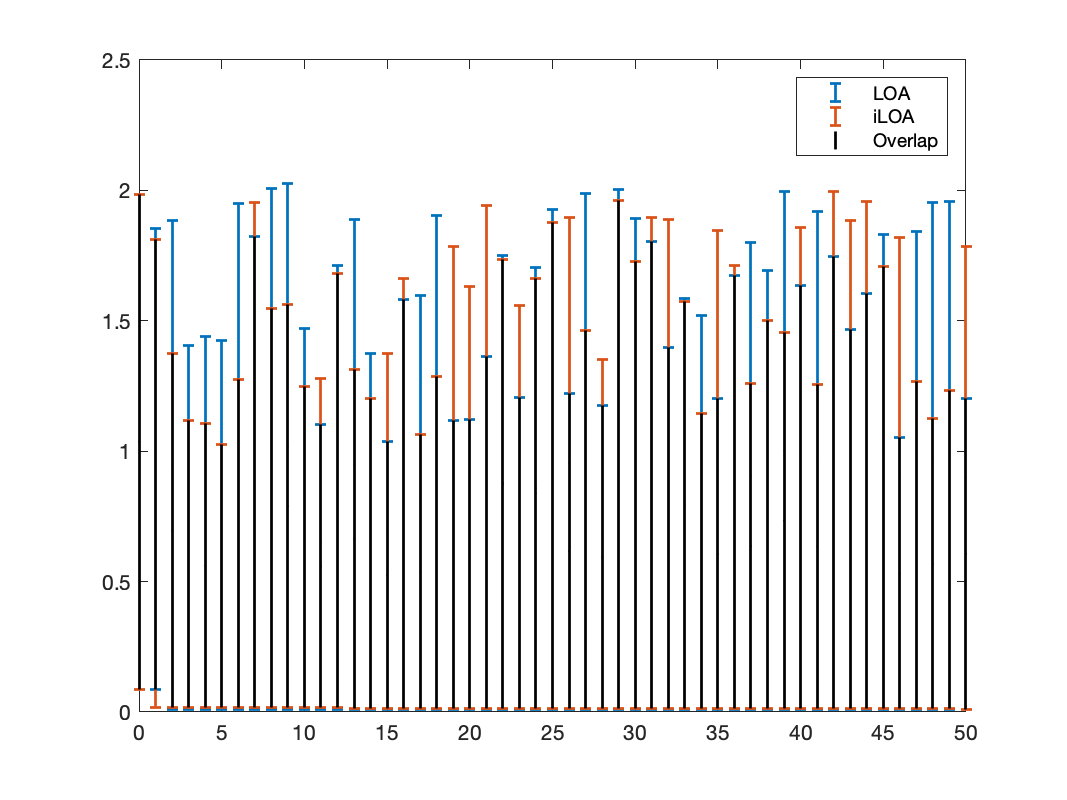
\includegraphics[width=\textwidth]{img/bars/f2/1}
    \caption{ \scriptsize Trial 1: Fitness Range (y) over Iterations (x)}
    \label{fig:f2-b-1}
  \end{subfigure}
  \begin{subfigure}[b]{0.4\textwidth}
    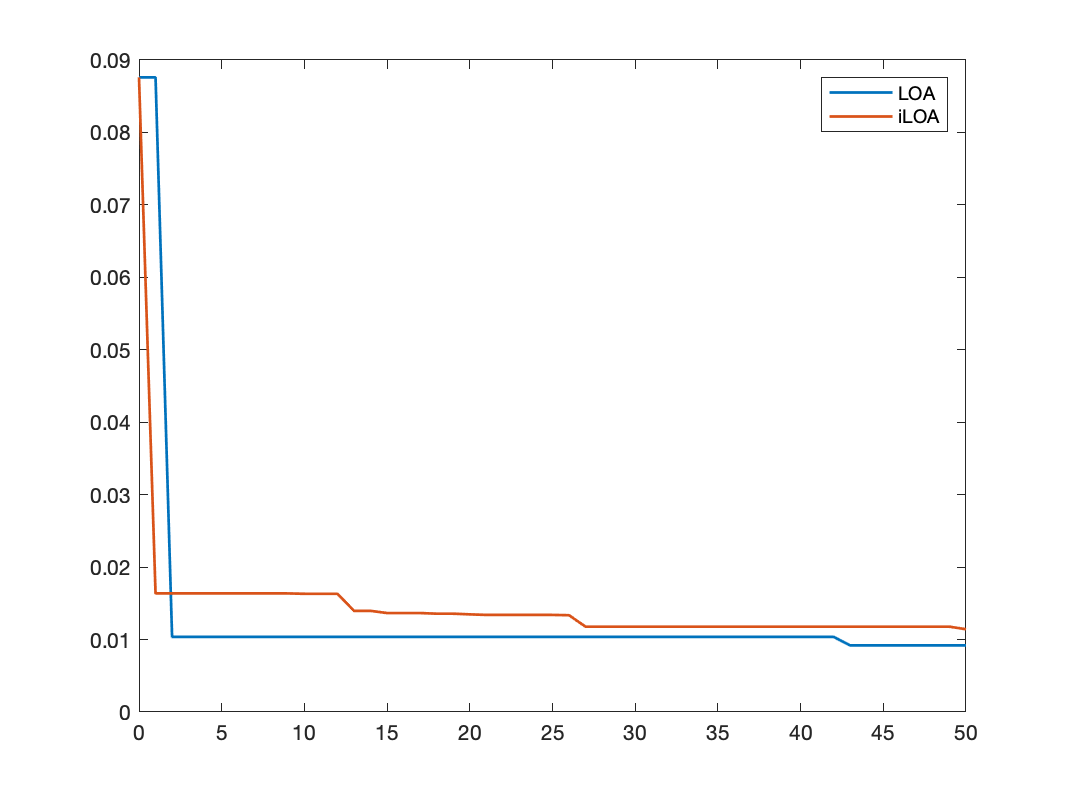
\includegraphics[width=\textwidth]{img/fits/f2/1}
    \caption{ \scriptsize Trial 1: Minimum Fitness (y) over Iterations (x)}
    \label{fig:f2-f-1}
  \end{subfigure}

  \begin{subfigure}[b]{0.4\textwidth}
    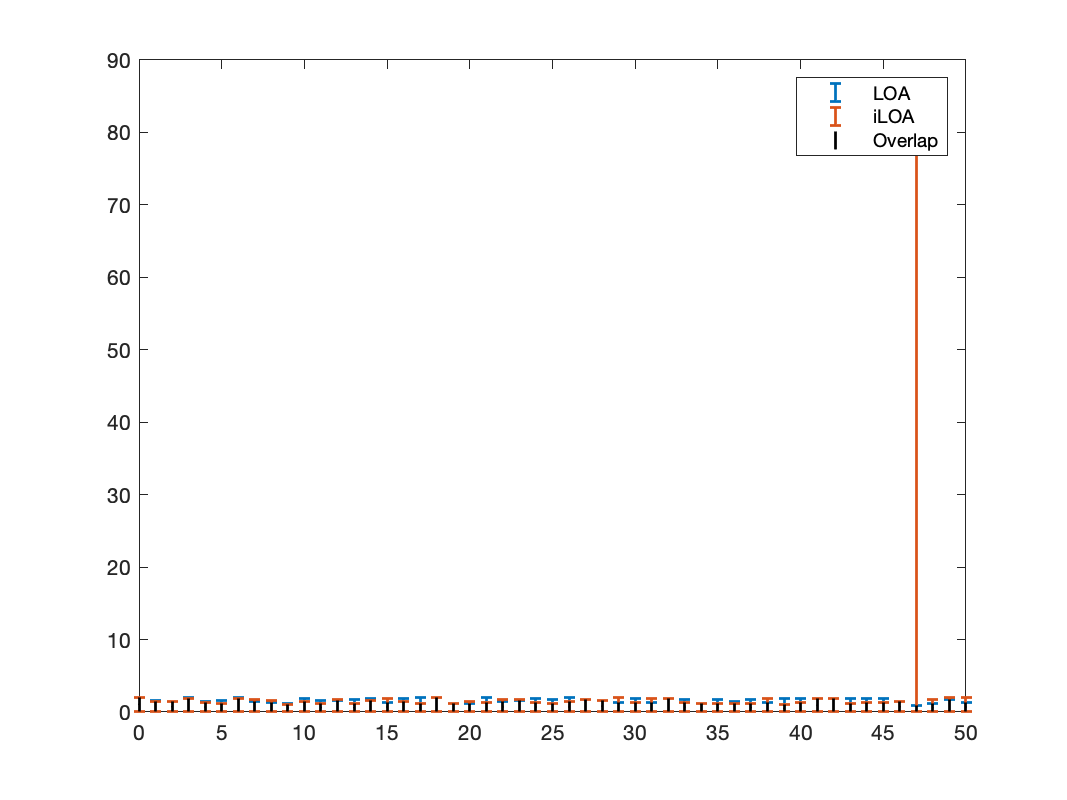
\includegraphics[width=\textwidth]{img/bars/f2/2}
    \caption{ \scriptsize Trial 2: Fitness Range (y) over Iterations (x)}
    \label{fig:f2-b-2}
  \end{subfigure}
  \begin{subfigure}[b]{0.4\textwidth}
    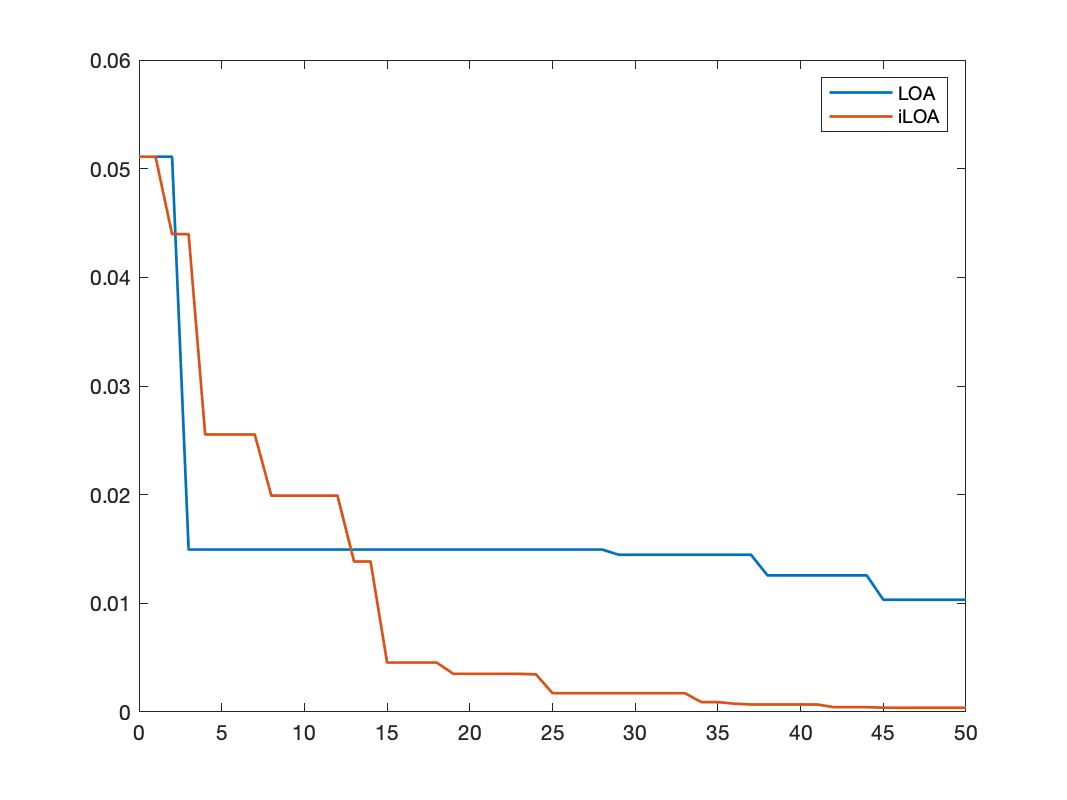
\includegraphics[width=\textwidth]{img/fits/f2/2}
    \caption{ \scriptsize Trial 2: Minimum Fitness (y) over Iterations (x)}
    \label{fig:f2-f-2}
  \end{subfigure}

  \begin{subfigure}[b]{0.4\textwidth}
    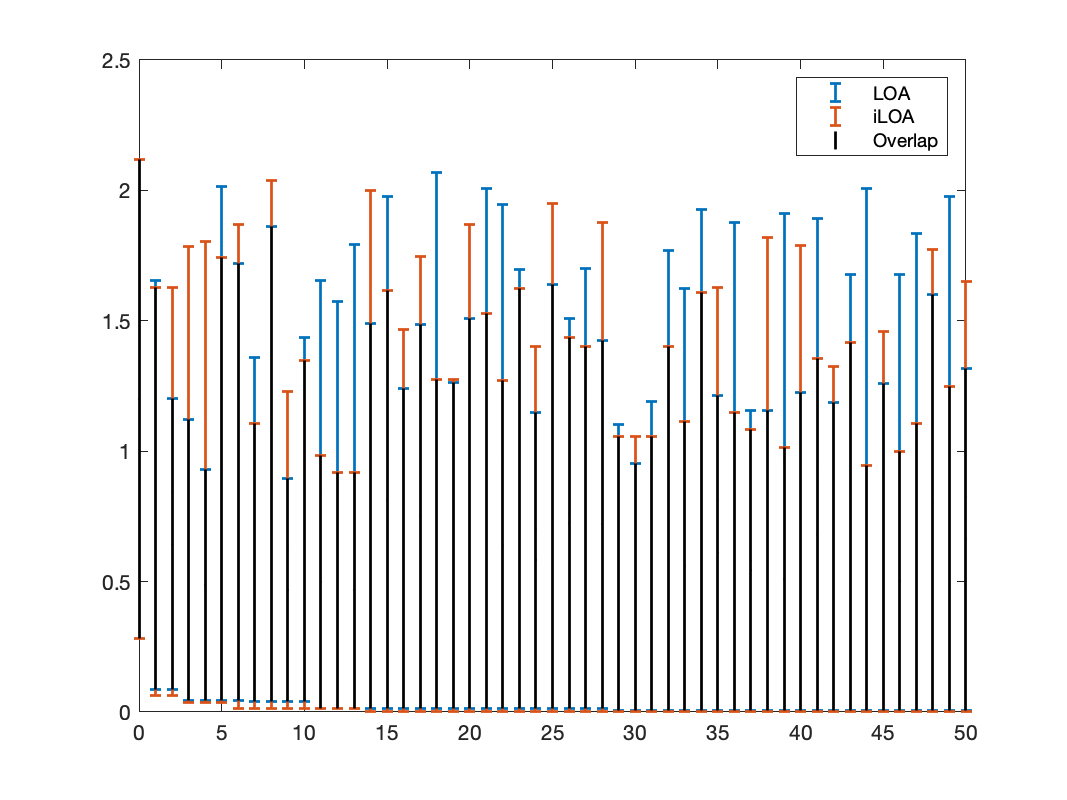
\includegraphics[width=\textwidth]{img/bars/f2/3}
    \caption{ \scriptsize Trial 3: Fitness Range (y) over Iterations (x)}
    \label{fig:f2-b-3}
  \end{subfigure}
  \begin{subfigure}[b]{0.4\textwidth}
    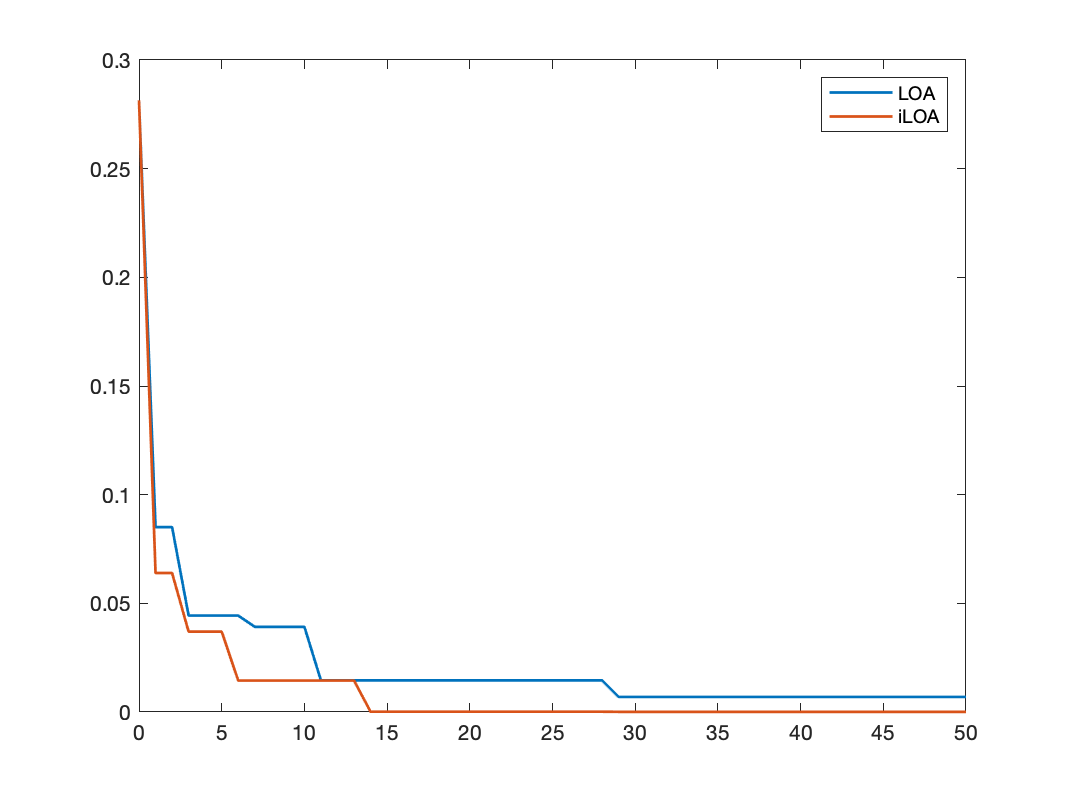
\includegraphics[width=\textwidth]{img/fits/f2/3}
    \caption{ \scriptsize Trial 3: Minimum Fitness (y) over Iterations (x)}
    \label{fig:f2-f-3}
  \end{subfigure}

  \begin{subfigure}[b]{0.4\textwidth}
    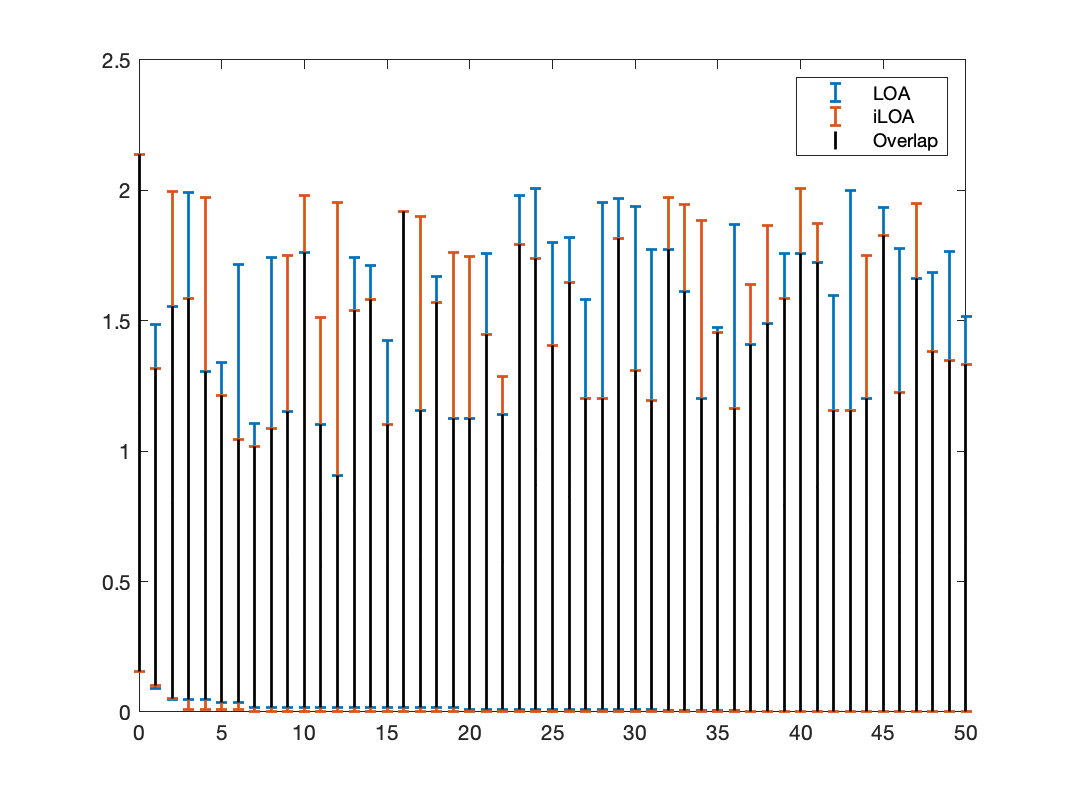
\includegraphics[width=\textwidth]{img/bars/f2/4}
    \caption{ \scriptsize Trial 4: Fitness Range (y) over Iterations (x)}
    \label{fig:f2-b-4}
  \end{subfigure}
  \begin{subfigure}[b]{0.4\textwidth}
    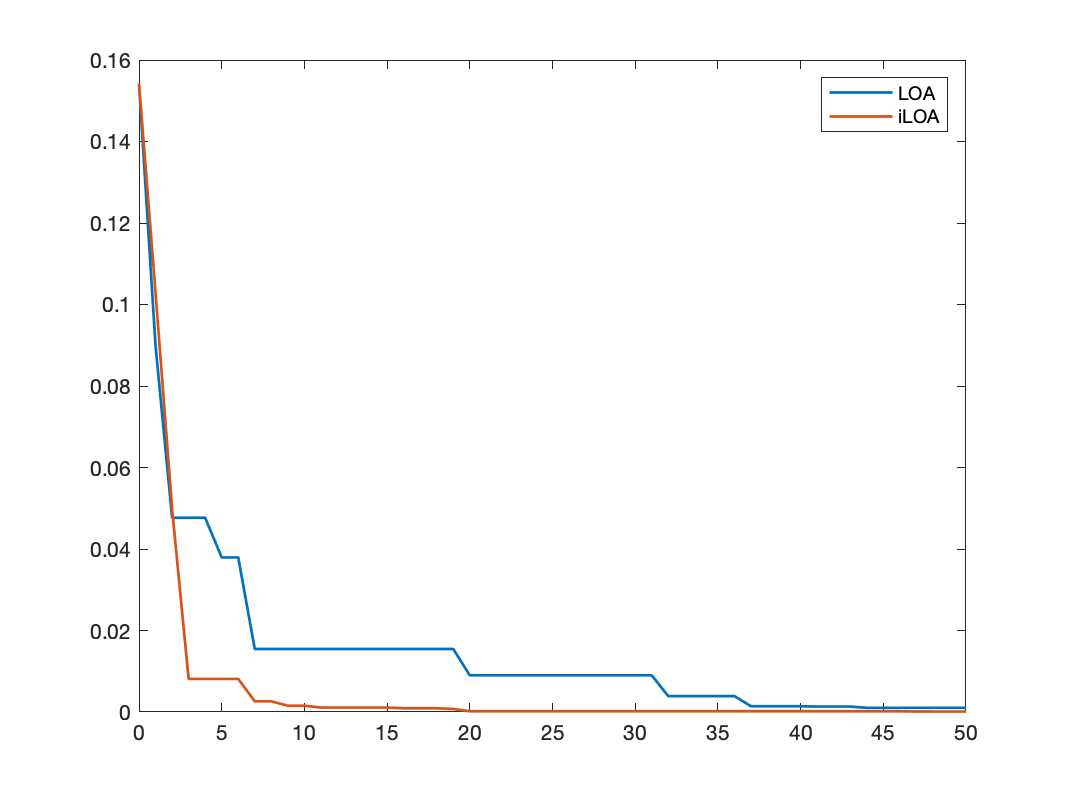
\includegraphics[width=\textwidth]{img/fits/f2/4}
    \caption{ \scriptsize Trial 4: Minimum Fitness (y) over Iterations (x)}
    \label{fig:f2-f-4}
  \end{subfigure}

  \begin{subfigure}[b]{0.4\textwidth}
    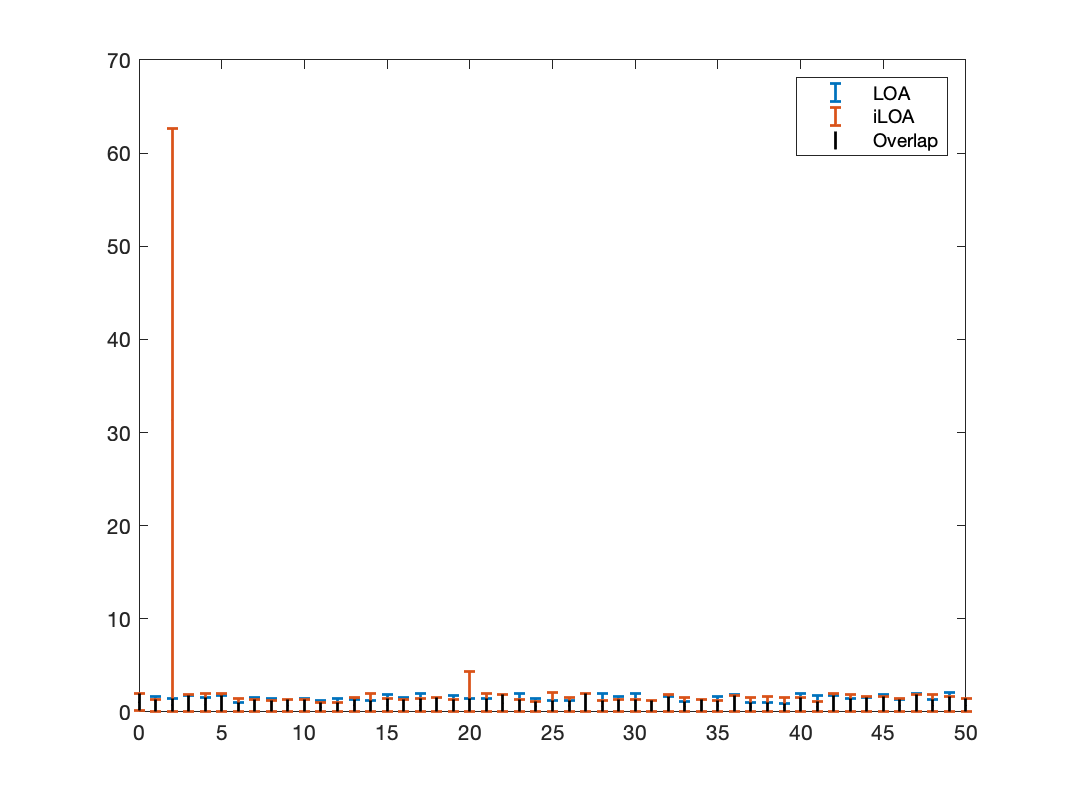
\includegraphics[width=\textwidth]{img/bars/f2/5}
    \caption{ \scriptsize Trial 5: Fitness Range (y) over Iterations (x)}
    \label{fig:f2-b-5}
  \end{subfigure}
  \begin{subfigure}[b]{0.4\textwidth}
    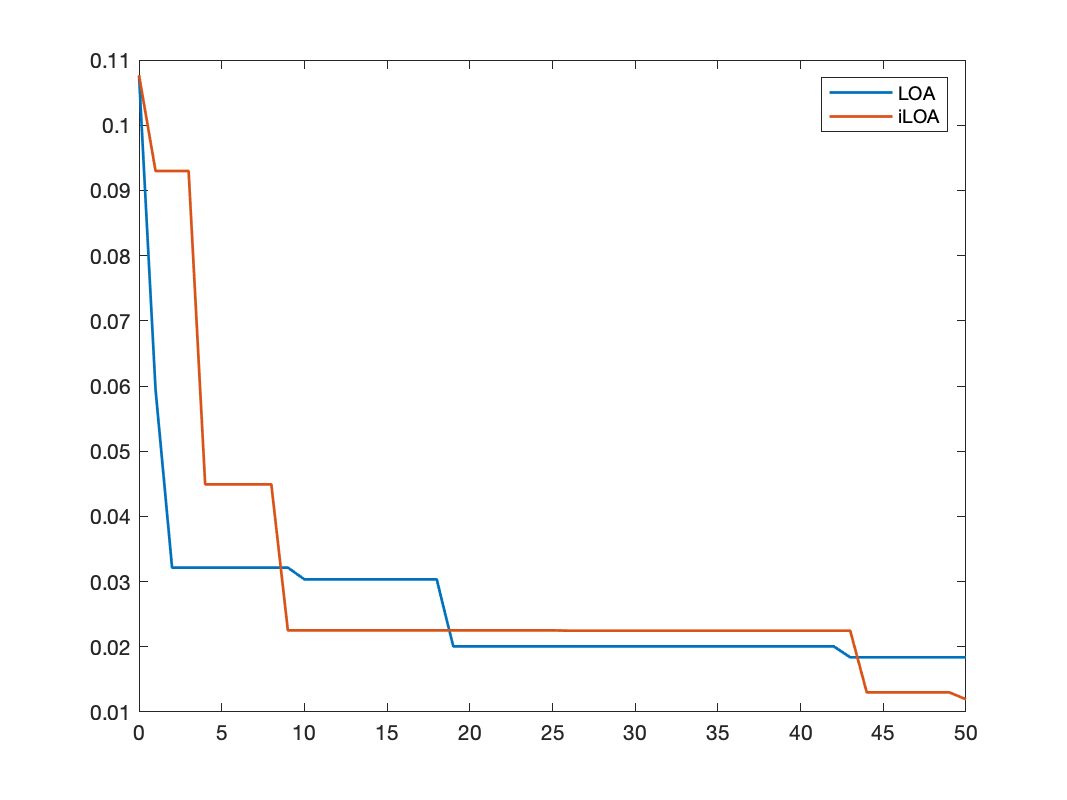
\includegraphics[width=\textwidth]{img/fits/f2/5}
    \caption{ \scriptsize Trial 5: Minimum Fitness (y) over Iterations (x)}
    \label{fig:f2-f-5}
  \end{subfigure}

  \caption{ \scriptsize LOA vs. iLOA: Griewank 2D ($f_2$)}
\end{figure}
